\section{Simulasi Monte Carlo}
\label{sec:montecarlo-simulation}

Simulasi Monte Carlo adalah teknik untuk memperkirakan nilai suatu fungsi ketika perhitungan langsung sulit atau tidak mungkin dilakukan. Teknik ini menggunakan sampling acak untuk menetapkan batasan pada nilai dan kemudian memberikan hasil yang mendekati. Kemajuan dalam komputasi telah merevolusi simulasi stokastik atau Monte Carlo. Dinamai menurut kasino perjudian Monte Carlo di Monaco, metode ini, yang juga dikenal sebagai metode percobaan statistik, menggabungkan teori probabilitas dari proses acak, seperti gerakan Brownian, dengan teori potensial, yang memeriksa keadaan keseimbangan dalam medium homogen. Metode ini menyelesaikan masalah secara mendekati menggunakan deret angka acak dengan menemukan analog probabilistik dan mendapatkan jawaban mendekati melalui sampling eksperimental \citep{Muqri_2020}.

Metode Monte Carlo dapat dikenali dari tiga karakteristik utamanya:

\begin{itemize}
    \item Pembuatan sampel yang acak
    \item Penentuan distribusi input yang diketahui
    \item Percobaan secara numerik
\end{itemize}

Output utama dari simulasi Monte Carlo adalah generasi sampel acak, sementara output kinerja atau statistik lainnya bergantung pada aplikasi spesifik. Berbagai percobaan numerik dapat dilakukan, termasuk distribusi probabilitas, yang mengidentifikasi kemungkinan setiap nilai dari variabel acak yang tidak diketahui (diskret) atau kemungkinan nilai tersebut jatuh dalam interval tertentu (kontinu). Untuk variabel acak kontinu, probabilitas dari nilai spesifik adalah nol. Contoh distribusi kontinu termasuk distribusi normal, seragam kontinu, beta, dan gamma \citep{Muqri_2020}.

Metode Monte Carlo sangat penting untuk menganalisis instrumen keuangan, portofolio, aset, berbagai jalur harga, dan perhitungan nilai opsi akhir. Metode ini unggul dalam menangani persamaan kompleks, membantu dalam perhitungan nilai yang tidak pasti, yang membantu dalam menganalisis nilai akhir dari instrumen atau aset. Karena nilai input juga bisa dikehendakai maka analis dapat melakukan percobaan sesuai dengan derajat keyakinan mereka atau memodelkan pendapatan sesuai dengan penanganan resiko yang mereka anut.

\begin{figure}[!ht]
    \centering
    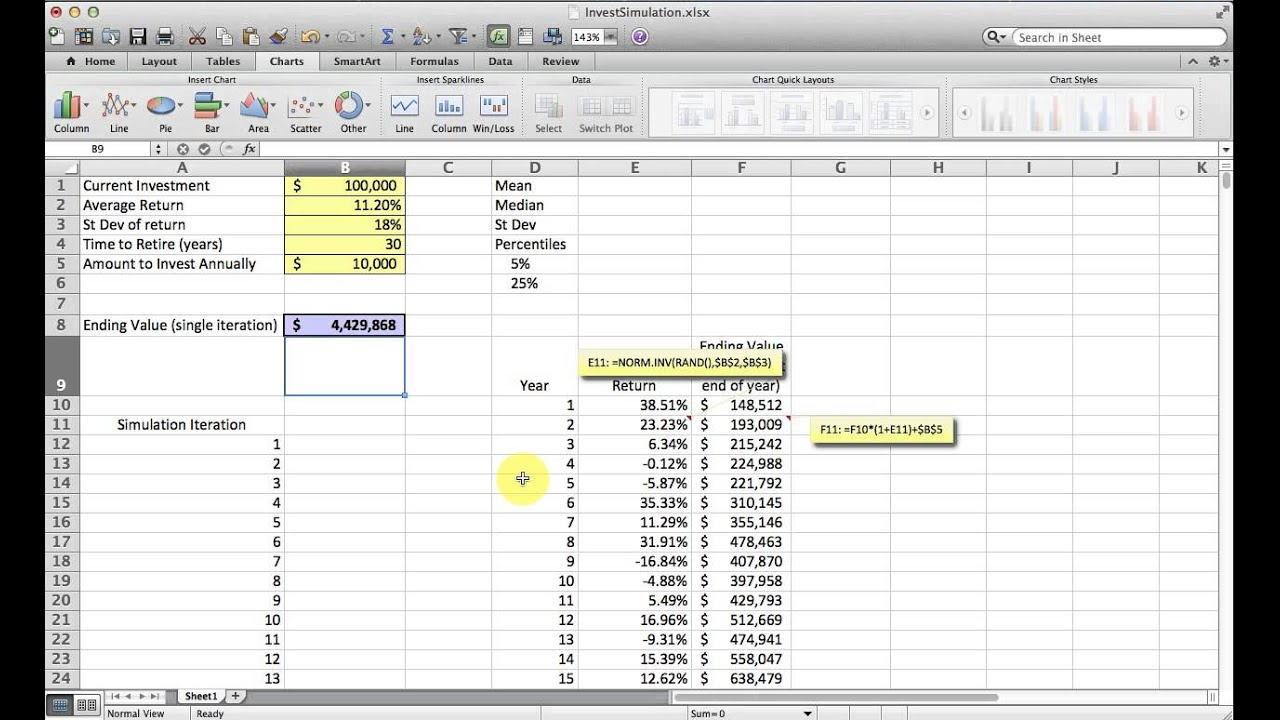
\includegraphics[width=0.8\textwidth]{gambar/excel-carlo.jpg}
    \caption{Penggunaan \emph{Microsoft Excel} untuk melakukan simulasi \citep{Matt_Macarty_2013}}
    \label{fig:ilustrasi-Excel-Carlo}
\end{figure}

\begin{figure}[h!]
    \centering
    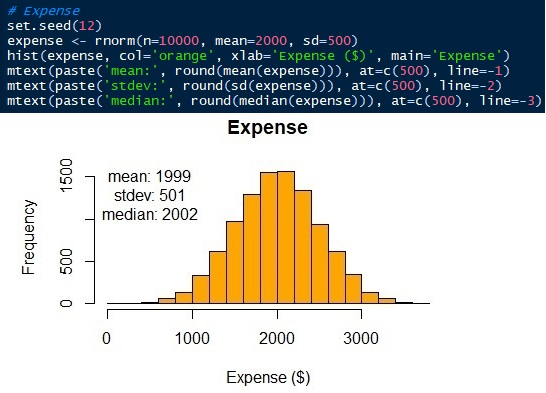
\includegraphics[width=0.8\textwidth]{gambar/r-carlo.jpg}
    \caption{Ilustrasi penggunaan Bahasa R untuk Simulasi \citep{Rendyk_2021}}
    \label{fig:R-monte-carlo}
\end{figure}

Simulasi Monte Carlo adalah alat yang tepat untuk memprediksi hasil masa depan dengan menghitung formula berulang kali dengan input acak yang berbeda. Penggunaan metode ini di bidang bisnis untuk memprediksi nilai masa depan dapat dilakukan dengan menghitung formula beberapa kali dengan input acak untuk saat ini dapat dilakukan di Excel dengan VBA atau plugin pihak ketiga, menggunakan alternatif seperti \emph{numpy} dan \emph{pandas} untuk membangun model dan menghasilkan berbagai hasil relatif mudah jika kita memiliki keterampilan dasar dalam bahasa Python. Selain itu, analis dapat menjalankan berbagai skenario dengan mengubah input, memungkinkan pemodelan yang lebih kompleks di masa depan sesuai kebutuhan.


